% =============================================================================
% Half-pager: sensor-interface pruning in the SoCal wildfire-grid co-simulation.
%
% Audience: the developer of this simulation. Context is deliberately thin --
% MIDAS, mosaik, palaestrAI and the SoCal grid are assumed known. If this is
% ever sent outside that audience, Section 1 needs two sentences of setup.
%
% Build:  cd paper && pdflatex whitelist_halfpager.tex   (twice, for the refs)
% Needs:  paper/fig_cost.pdf  (regenerate: python analysis/cost_figure.py)
%
% ONE page including both figures. If you add text, take some out: Limitations
% compresses first, then the ordering property in Section 3.
% =============================================================================
\documentclass[10pt,a4paper]{article}

\usepackage[top=1.7cm,bottom=1.7cm,left=1.9cm,right=1.9cm]{geometry}
\usepackage{microtype}
\usepackage{amsmath}
\usepackage{graphicx}
\usepackage{booktabs}
\usepackage{wrapfig}
\usepackage{tikz}
\usetikzlibrary{arrows.meta,positioning,fit,backgrounds}
\usepackage[hidelinks]{hyperref}
\usepackage{titlesec}
\usepackage{enumitem}
\usepackage{caption}
% Default Computer Modern: this TeX Live has neither newtx nor the Times TFMs.
% On a fuller installation add:
%   \usepackage[T1]{fontenc}\usepackage{newtxtext,newtxmath}

\titlespacing*{\section}{0pt}{0.9ex plus .1ex}{0.35ex}
\titleformat{\section}{\normalfont\bfseries\large}{\thesection.}{0.5em}{}
\setlist[itemize]{nosep,leftmargin=1.2em,topsep=2pt}
\captionsetup{font=small,labelfont=bf,skip=3pt}
\setlength{\parskip}{0.2ex}
\pagestyle{empty}

\newcommand{\x}{$\times$}

\begin{document}

\begin{center}
  {\large\bfseries Pruning the ARL Sensor Interface: a 6.7\x{} Per-Step Speedup\\[2pt]
   with Bit-Identical Trajectories}\\[4pt]
  {\small Josef Leinweber, Jonas Bock \quad\textbullet\quad Integrated Energy Systems}
\end{center}
\vspace{-0.5em}

\section{The cost}
The \texttt{socal\_grid} environment advertises \textbf{66{,}223 sensors and
11{,}250 actuators}: 9{,}637 pandapower elements (2{,}294 buses, 2{,}595 lines,
2{,}465 sgens, 1{,}932 loads, 345 transformers) at roughly seven attributes
each. This follows from the grid model and the \texttt{powergrid} module, so
every experiment in the repository sees it. Agents subscribe to \textbf{31}; the
remaining 99.95\,\% are built, serialised, shipped across the message bus and
discarded, once per step, for the whole of training.

\section{Where the filtering happens}
\begin{center}
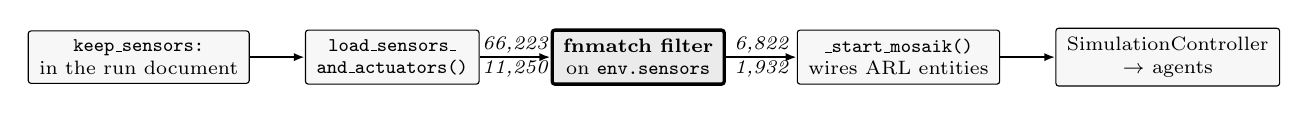
\begin{tikzpicture}[
  font=\scriptsize,
  node distance=0pt,
  box/.style={draw,rounded corners=1pt,minimum height=5.2mm,inner xsep=4pt,
              align=center,fill=black!3},
  cut/.style={draw,very thick,rounded corners=1pt,minimum height=5.2mm,
              inner xsep=4pt,align=center,fill=black!8},
  ar/.style={-{Latex[length=1.4mm]},thick},
  lbl/.style={font=\scriptsize\itshape,inner sep=1pt}
]
\node[box] (yaml) {\texttt{keep\_sensors:}\\ in the run document};
\node[box,right=7mm of yaml] (load) {\texttt{load\_sensors\_}\\\texttt{and\_actuators()}};
\node[cut,right=9mm of load] (filt) {\textbf{fnmatch filter}\\ on
  \texttt{env.sensors}};
\node[box,right=9mm of filt] (wire) {\texttt{\_start\_mosaik()}\\ wires ARL
  entities};
\node[box,right=7mm of wire] (agent) {SimulationController\\ $\rightarrow$ agents};

\draw[ar] (yaml) -- (load);
\draw[ar] (load) -- node[lbl,above] {66{,}223} node[lbl,below] {11{,}250} (filt);
\draw[ar] (filt) -- node[lbl,above] {6{,}822} node[lbl,below] {1{,}932} (wire);
\draw[ar] (wire) -- (agent);
\end{tikzpicture}
\end{center}
\vspace{-0.6em}

The filter runs \emph{between} enumeration and entity creation: a pruned sensor
is never wired, stepped or serialised, so the cost is not reduced but never
incurred. Two properties make this safe rather than merely fast. palaestrAI
validates every agent subscription against the advertised sensors at setup and
raises before the first step, so a run that starts has full agent observability
\emph{by construction} --- the filter can abort a run, never silently starve a
learner. And it preserves the survivors' relative order, so summation order in
reward computation, and hence its floating-point result, is unchanged.

\section{Validation}
Four arms were generated from one source run document by one documented mutation
each, then run for four scripted phases \x{} 60 steps. At every step we compared
the SHA-256 of the fire raster, the structural telemetry and all 1{,}932 load
sensors, reporting the number of cells whose state differs. Agreement is exact,
not within a tolerance.

\textbf{The \texttt{grid\_probe} agent was removed from every arm.} Its
\texttt{DummyMuscle} writes \texttt{actuator.space.sample()} into
\texttt{Powergrid-0.0-load-0-0.p\_mw}: a random active-power setpoint each step,
from a gymnasium \texttt{Box} seeded from OS entropy. With it present, two
byte-identical configurations diverge and no comparison means anything.

\vspace{0.25em}
\begin{center}
\small
\begin{tabular}{@{}llr@{}}
\toprule
& \textbf{Arms differ by} & \textbf{Cells differing}\\
\midrule
Reproducibility control & nothing (identical configurations) & \textbf{0}\\
\textbf{Treatment}      & the filter, on vs.\ off            & \textbf{0}\\
Sensitivity control     & fire wind speed $+3.6\,\%$         & 360\\
\bottomrule
\end{tabular}
\end{center}
\vspace{-0.15em}

The sensitivity control perturbs the fire driver's \texttt{base\_speed}
($14 \rightarrow 14.5$\,m/s) with terrain held identical, and must diverge. It is
what gives the two zeros meaning: without it, ``identical'' reported twice is
equally consistent with a comparison that detects nothing. Arms were compared as
\emph{stored} run documents rather than configuration files --- treatment and
baseline differ in exactly ten leaves: two identifiers, and the filter entries in
each of the four phases.

\section{Result}
\begin{wrapfigure}{r}{0.35\textwidth}
  \vspace{-1.5em}
  \centering
  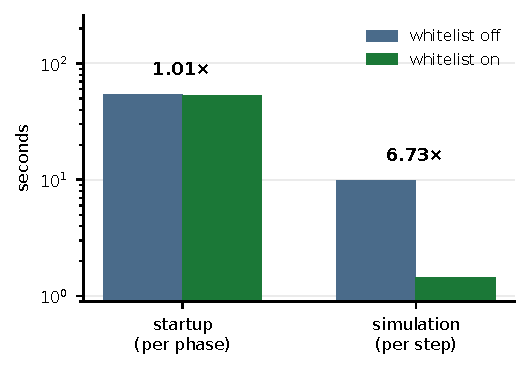
\includegraphics[width=\linewidth]{fig_cost.pdf}
  \caption{The gain is confined to the per-step term; fixed startup is
  untouched.}
  \label{fig:cost}
  \vspace{-1.4em}
\end{wrapfigure}
Running each arm at two lengths (8 and 60 steps) determines
$\text{total}=4\,(\text{startup}+\text{steps}\times\text{per\_step})$ exactly,
separating fixed from marginal cost (Fig.~\ref{fig:cost}). Per-step cost falls
from $9.77$\,s to $1.45$\,s, a factor of \textbf{6.73}; per-phase startup is
unchanged ($53.8 \rightarrow 53.4$\,s). Noise between two bit-identical runs was
$0.6\,\%$, so this is not a scheduling artefact. Because fixed cost is untouched,
any end-to-end ratio depends on episode length and understates the effect.

\section{Limitations}
Scripted policies only: the DRL phases still contain \texttt{grid\_probe}, so
they are not reproducible against themselves and bit-comparison does not apply;
equivalence for learners rests on Section~2. The store retains only load sensors
(identically in both arms), so equivalence is established on the
outcome-relevant projection. One scenario, one seed.

\section{Reproducing this}
\vspace{-0.3em}
{\small\setlength{\baselineskip}{9pt}
\begin{verbatim}
python analysis/make_whitelist_configs.py  # arms, from one source document
./run_whitelist_validation.sh              # ~2 h: all arms, both controls
python analysis/cost_figure.py             # Figure 1
\end{verbatim}}
\vspace{-0.9em}
The runner aborts before reporting the treatment if the reproducibility control
diverges or the sensitivity control does not, and refuses to start if the arm
documents have drifted from the generator. Each arm keeps its own database
(\texttt{analysis/compare\_runs.py}).

\end{document}
